\documentclass[10pt]{beamer}
\DeclareOptionBeamer{compress}{\beamer@compresstrue}
\ProcessOptionsBeamer
\mode<presentation>{}
\usetheme{Boadilla}
\usepackage[utf8]{inputenc}
\usepackage{amsmath}
\usepackage{amsfonts}
\usepackage{amssymb}
\usepackage{hyperref}
\hypersetup{
    colorlinks=true,
    linkcolor=cyan!60!white,
    filecolor=magenta,
    urlcolor=cyan,
    pdftitle={Sharelatex Example},
    bookmarks=true,
    pdfpagemode=FullScreen,
}
\usepackage{graphicx}
\usepackage[style=alphabetic,citestyle=authoryear,backend=bibtex]{biblatex}
\bibliography{biblio.bib}
\author[SN, MA, AGB]{\hspace*{1.5em} Soham Naha \hfill \and Mohit Agarwala \hfill \and Abhinav Goud Bingi\\ \textsc{ (193079003) \hfill \and (19307R004) \hfill \and (180050002)}}

\institute[IITB]{Indian Institute of Technology, Bombay \\ 
\includegraphics[height=2cm,width=2cm]{images/iitb_logo.png}}
\title[CS 753 Project]{CS 753 Project\\{\normalsize Speech to Sign-Language(with emotions) for the Hearing-Impaired}}
\setbeamercovered{transparent} 
\setbeamertemplate{navigation symbols}{} 
%\logo{images/iitb_logo.png}
%\institute[IITB]{Indian Institute of Technology, Bombay} 
%\date{} 
%\subject{} 
\begin{document}
\begin{frame}
\titlepage
\end{frame}

\begin{frame}
\tableofcontents
\end{frame}

\AtBeginSection[]
{
\begin{frame}
	\frametitle{Table of Contents}
	\tableofcontents[currentsection]
\end{frame}
}

\section{Problem Definition}
\begin{frame}{Problem Statement}
Given a speech utterence from a speaker who is trying to convey a message to a person who is hearing-impaired and/or voiceless, then speech has to be converted in a form that the other person can understand, i.e. in a sign language.
\end{frame}

\section{Motivation}
\begin{frame}
\begin{itemize}
	\item Most of the literature in the field of ASL and Speech are based on the conversion of sign-to-speech.
	\item But the converse model that completes the cycle of sign-to-speech, i.e. speech-to-sign, is mostly unexplored.
	\item In this project, we explore the speech-to-sign paradigm Deep Learning ASR models.
	\item This project could be used as a conversation model for the speech and/or hearing-impaired to interact with people who dont have knowledge of sign-language.
\end{itemize}
\end{frame}

\section{Subtasks}
\begin{frame}{Subtasks}
\begin{itemize}
	\item Speech to text conversion (ASR)
	\item Speech to emotion recognition
	\item Text to Sign Language Conversion (Future Work)
\end{itemize}
\end{frame}

\section{Speech to text conversion}
\begin{frame}{Task1: Speech to Text}
\begin{itemize}
	\item The speech2text problem is one of the most classical problems in ASR.
	\item It started from a statistical modelling problem with separate model components like the acoustic model, language model and the pronunciation model.
	\item On the advent of the era of Deep Learning, this changed to an End-to-End modelling paradigm.
	\item It started with Tandem and Hybrid networks, with the present state-of-the-art(SOTA) model being the Conformer-based model.
\end{itemize}
\end{frame}

\begin{frame}{Task1: Speech to Text}
\begin{itemize}
	\item Dataset: LIBRISPEECH \footcite{librispeech}
	\item We initially wanted to train our own Speech2Text network using a CTC-Beam Search based CNN-LSTM model.
	\item But due to constraint in resources could not train the model.(code is present but only able to run 30 epochs over 4days)	
	\item So, we reverted to the ESPNet Toolkit\footcite{espnet}.
	\item From this toolkit we used the model \href{https://zenodo.org/record/4604011}{here} %\footcite{espnet_model}.
	\item It uses a conformer based architecture for the acoustic model and a transformer based architecture for the language model.
	\item We have used the pre-trained models for both.
	\item The metrics claimed by the model on \texttt{test-clean} are:
	\begin{center}
	\begin{tabular}{|c|c|c|c|c|}
	\hline
	Metric & Sub & Del & Ins & Err \\
	\hline
	WER & 2.1 & 0.2 & 0.3 & 2.6 \\
	CER & 1.2 & 0.8 & 0.7 & 2.7 \\
	\hline
	\end{tabular}
	\end{center}
	
\end{itemize}
\end{frame}

\section{ESPNet Model}
\begin{frame}{Short Description of ESPNet Architecture }
The Conformer-based model architecture \footcite{espnet} is as follows:
\begin{itemize}
	\item The input speech signal is converted into a sequence of 80 dimensional log-mel filterbank features with/without 3-dimensional pitch features.
	\item Then, passed through a Conformer-based encoder.
	\item The output of the above block is passed through a Transformer-based decoder.
	\item The encoder-decoder model was trained using joint-CTC-attention training and decoding.
	\item Followed by a token/word-level language model (transformer based) via shallow fusion.
\end{itemize}
\end{frame}

\section{Emotion Recognition}
\begin{frame}{Emotion Recogition}
\begin{itemize}
	\item \textbf{Motivation}:\\
	Often the emotion carried out by an utterence cannot be properly conveyed using sign-language.
	\item \textbf{Dataset}: RAVDESS \footcite{ravdess}
	\item Data Pre-processing:
	\begin{itemize}
		\item Convert the input speech signal into 128-dimensional Mel-Spectogram
	\end{itemize}
	\item Model:
	\begin{itemize}
		\item The model used is a CNN-based model with a softmax layer, trained on Sparse Categorical Cross-Entropy Loss.
		\item Model Accuracy: $72\%$
		
	\end{itemize}
\end{itemize}
\end{frame}

\section{Text to Sign Language Conversion}
\begin{frame}{Text to Speech Conversion}
\begin{itemize}
	\item We thought of building a speech to sign-language tool, by first converting the speech to text and for every word map to american sign-language (ASL) representation.
	\item \textcolor{red!60!white}{**Disclaimer:
{\small We could not implement the text ot sign language part.}}
	\item We came across several datasets that converted the letters to ASL hand-images, but that was not what we intended.
	\item There were other Unity and Blender based Avatar models, but that were not truly capable of direct text to ASL conversion, because of limited datasets.
	\item We got an architecture that treated this problem as a \href{https://github.com/arunnair411/Speech-to-ASL}{GAN-based model}, but we could not implement  it due constraints.
	\item The Workflow was as follows:
	\begin{itemize}
		\item Translate text to ASL glossary using Transformer model.
		\item Align the ASL Glossary to poses using OpenPose.
		\item Interpolate the poses generated using a Fully-Connected neural network (FCN).
		\item Generate avatar images for each pose using pix2pix GAN and compile as a video.
	\end{itemize}
\end{itemize}
\end{frame}


\section{Tool Developed}
\begin{frame}{Web Tool for the pipeline}
\begin{itemize}
	\item We created a toolkit using the \texttt{streamlit} module of python where we can record a 10sec audio and can detect text and emotion.
\end{itemize}
\begin{minipage}{0.3\textwidth}
\centering
\begin{figure}
	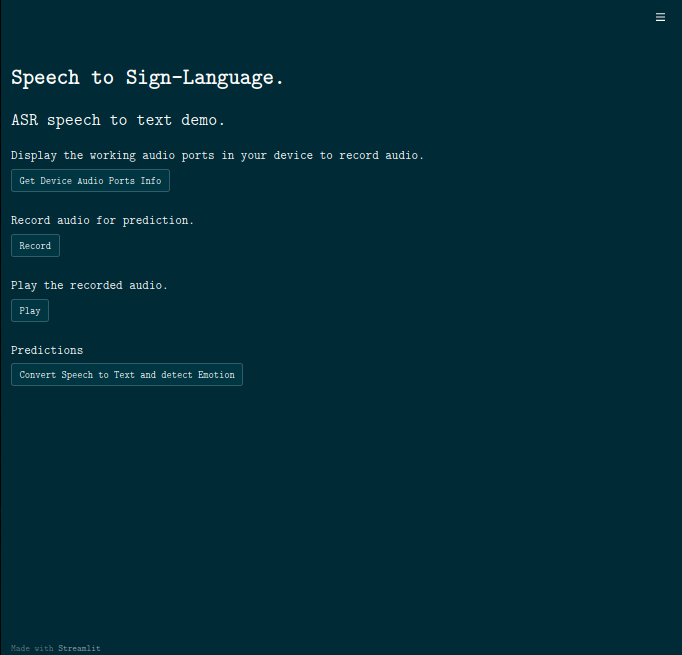
\includegraphics[width=\textwidth]{images/streamlit_app1.png}
	\caption{The Tool Overview}
\end{figure}
\end{minipage}
\begin{minipage}{0.3\textwidth}
\centering
\begin{figure}
	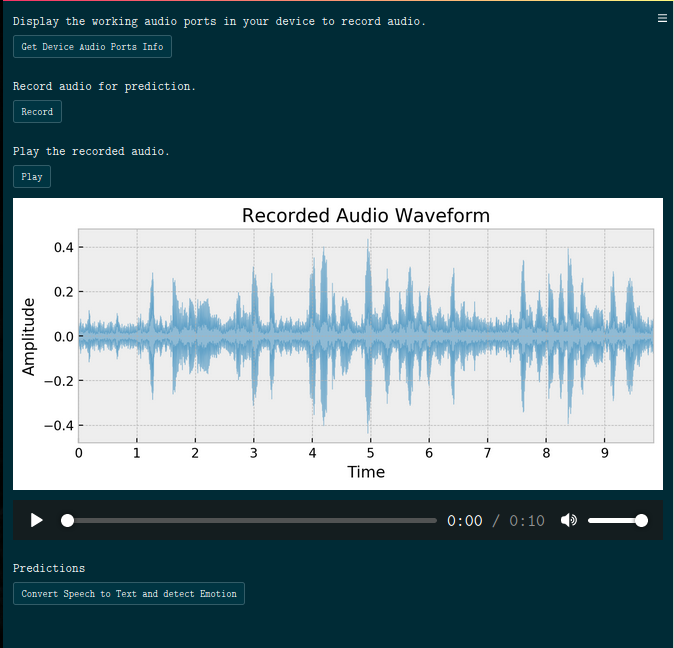
\includegraphics[width=\textwidth]{images/streamlit_app2.png}
	\caption{Play the Audio}
\end{figure}
\end{minipage}
\begin{minipage}{0.35\textwidth}
\centering
\begin{figure}
	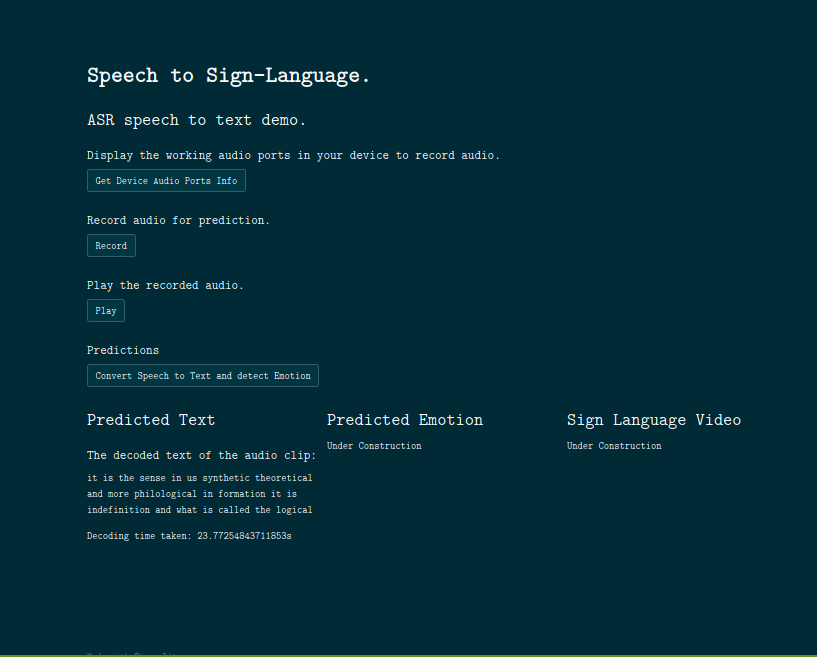
\includegraphics[width=\textwidth]{images/streamlit_app3.png}
	\caption{Audio Decoding}
\end{figure}
\end{minipage}

The accuracy of the toolkit depends on the accuracy of the models in general and we hope to integrate the text to ASL feature in future.
\end{frame}
		 
\section{References}
\begin{frame}{References}
	\tiny    
    \printbibliography
\end{frame}

\end{document}